\title{CS 613 - Machine Learning}
\author{Assignment 3 - Classification)\\ 	Alex Lapinski\\ 	Fall 2016}
\date{11/6/2016}
\documentclass[12pt]{article}
\usepackage[margin=0.7in]{geometry}
\usepackage{graphicx}
\usepackage{float}
\usepackage{comment}
\usepackage{amsmath}
\graphicspath{ {images/} }

\begin{document}
\maketitle
\section{Theory}
\begin{enumerate}
\item Consider the following set of training examples for an unknown target function:  $(x_1, x_2)\rightarrow y$:
\begin{table}[h]
\begin{center}
\begin{tabular}{|l|l|l|l|}
\hline
Y & $x_1$ & $x_2$ & Count\\
\hline
+ & T & T & 3\\
+ & T & F & 4\\
+ & F & T & 4\\
+ & F & F & 1\\
- & T & T & 0\\
- & T & F & 1\\
- & F & T & 3\\
- & F & F & 5\\
\hline
\end{tabular}
\end{center}
\end{table}
\begin{enumerate}
\item What is the sample entropy, $H(Y)$ from this training data (using log base 2) (2pts)?
\hfill \linebreak
\hfill \linebreak
Number of samples with '+' class (p): 12\\
Number of samples with '-' class (n): 9\\
Total number of samples (p+n): 21\\
\hfill \linebreak
\begin{equation*}
\begin{split}
		H(\frac{p}{p+n},\frac{n}{p+n})  & = H(\frac{12}{21},\frac{9}{21}) \\
		& = (-\frac{12}{21}*log_2(\frac{12}{21}) + (-\frac{9}{21}*log_2\frac{9}{21})) \\
		& = (-0.57*log_2(0.57)) + (-0.43log_2(-0.43)) \\
	         & = (-0.57*-0.81) + (-0.43 * -1.22) \\
		& = 0.46 + 0.52 \\
		& = \textbf{0.98}
\end{split}
\end{equation*}
\newpage
\item What are the information gains for branching on variables $x_1$ and $x_2$ (4pts)?
\hfill\linebreak
\hfill\linebreak
We'll first compute the information gain on $x_1$ and then on $x_2$.\\
The count for each class when split on $x_1$:
\begin{align*}
	p_{T} &= 3 + 4 = 7 & n_{T} &= 0 + 1 = 1 & p_{T} + n_{T} & = 8\\
	p_{F} &= 4 + 1 = 5 & n_{F} &= 3 + 5 = 8 & p_{F} + n_{F} & = 13 \\
	p+n &= 21 & &\\
\end{align*}
\begin{equation*}
\begin{split}
remainder(x_1) & = \frac{p_T + n_T}{p + n} * H(\frac{p_T}{p_T+n_T},\frac{n_T}{p_T+n_T}) + 
			     \frac{p_F+n_F}{p+n}*H(\frac{p_F}{p_F+n_F},\frac{n_F}{p_F+n_F})\\
	& = \frac{8}{21}*H(\frac{7}{8},\frac{1}{8}) + \frac{13}{21}*H(\frac{5}{13},\frac{8}{13})\\
	& = \frac{8}{21}*(-\frac{7}{8}*log_{2}(\frac{7}{8})-\frac{1}{8} * log_{2}(\frac{1}{8})) + 
	       \frac{13}{21}*(-\frac{5}{13}*log_{2}(\frac{5}{13})-\frac{8}{13}*log_{2}(\frac{8}{13}))\\
	& = \frac{8}{21}*(0.17+0.38) + \frac{13}{21}*(0.52+0.43)\\
	& = 0.21 + 0.59 = \textbf{0.8}\\
	\end{split}
\end{equation*}
\begin{equation*}
	IG(x_{1}) = 0.98 - 0.8 = \textbf{0.18}
\end{equation*}
\hfill\linebreak
The count for each class when split on $x_2$:
\begin{align*}
		p_{T} &= 3 + 4 = 7 & n_{T} &= 0 + 3 = 3 & p_{T} + n_{T} & = 10\\
		p_{F} &= 4 + 1 = 5 & n_{F} &= 1 + 5 = 6 & p_{F} + n_{F} & = 11\\
		p+n &= 21 & &\\
\end{align*}
\begin{equation*}
\begin{split}
	remainder(x_2) & = \frac{p_T + n_T}{p + n} * H(\frac{p_T}{p_T+n_T},\frac{n_T}{p_T+n_T}) + 
				      \frac{p_F+n_F}{p+n}*H(\frac{p_F}{p_F+n_F},\frac{n_F}{p_F+n_F})\\
	& = \frac{10}{21}*H(\frac{7}{10},\frac{3}{10}) + \frac{11}{21}*H(\frac{5}{11},\frac{6}{11})\\
	& = \frac{10}{21}*(-\frac{7}{10}*log_{2}(\frac{7}{10})-\frac{3}{10} * log_{2}(\frac{3}{10})) + 
	       \frac{11}{21}*(-\frac{5}{11}*log_{2}(\frac{5}{11})-\frac{6}{11}*log_{2}(\frac{6}{11}))\\
	& = \frac{10}{21}*(0.36+0.54) + \frac{11}{21}*(0.51+0.48)\\
	& = 0.43 + 0.52 = \textbf{0.85}\\
\end{split}
\end{equation*}
\begin{equation*}
	IG(x_{2}) = 0.98 - 0.85 = \textbf{0.13}
\end{equation*}
\hfill\newline
\newpage
\item Draw the decision tree that would be learned by the ID3 algorithm without pruning from this training data (5pts)?
\\
\begin{figure}[h]
\caption{Initial Decision Tree, where leaf nodes are not collapsed}
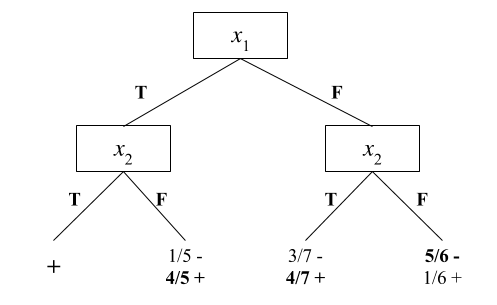
\includegraphics[width=10cm]{InitialTree}
\centering
\end{figure}
\begin{figure}[h]
\caption{Final Decision Tree, collapsed left node, select most probable outcome for other nodes.}
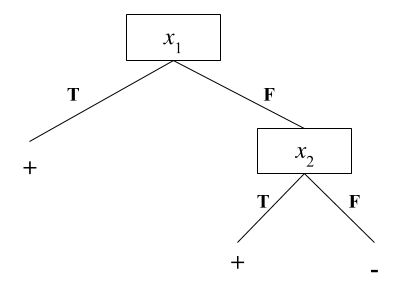
\includegraphics[width=10cm]{FinalTree}
\centering
\end{figure}
\newpage
\end{enumerate}
	
\item We decided that maybe we can use the number of characters and the average word length an essay to determine if the student should get an $A$ in a class or not.  Below are five samples of this data:
\begin{table}[h]
\begin{center}
\begin{tabular}{|l|l|l|}
\hline
\# of Chars & Average Word Length & Give an A\\
\hline
216 & 5.68 & Yes\\
69 & 4.78 & Yes\\
302 & 2.31 & No \\
60 & 3.16 & Yes \\
393 & 4.2 & No\\
\hline
\end{tabular}
\end{center}
\end{table}
\begin{enumerate}
\item What are the class priors, $P(A=Yes), P(A=No)$? (1pt)
\item Find the parameters of the Gaussians necessary to do Gaussian Naive Bayes classification on this decision to give an A or not.  Standardize the features first over all the data together so that there is no unfair bias towards the features of different scales (5pts).
\item Using your response from the prior question, determine if an essay with 242 characters and an average word length of 4.56 should get an A or not (5pts).
\end{enumerate}
\item Consider the following questions pertaining to a k-Nearest Neighbors algorithm (1pt each = 3pts):
\begin{enumerate}
\item How could you use a \emph{validation set} to determine the user-defined parameter $k$?
\item Why shouldn't you use the training set to determine this?
\item Why shouldn't you use the testing set to determine this?
\end{enumerate}
\item The Linear Kernel is commonly used if we already are working in high feature space.  It is defined as $k(x,y)=\sum_{d=1}^D x_d y_d$.  If your observations have three features ($D=3$), what is the function $\phi(u)$ such that $k(x,y)=\phi(x)\phi(y)$?  Show your work (4pts).
\item True or false:  A Gaussian Kernel is better than a linear kernel when there are many features but few training samples (1pt).
\end{enumerate}

\newpage
\section{Naive Bayes Classifier}\label{naive}
Let's train and test a \emph{Naive Bayes Classifier} to classifiy Spam or Not from the Spambase Dataset.\\

\noindent
First download the dataset \emph{spambase.data} from Blackboard.  As mentioned in the Datasets area, this dataset contains 4601 rows of data, each with 57 continuous valued features followed by a binary class label (0=not-spam, 1=spam).  There is no header information in this file and the data is comma separated.  As always, your code should work on any dataset that lacks header information and has several comma-separated continuous-valued features followed by a class id $\in {0,1}$.\\

\noindent
\paragraph{Write a script that:}
\begin{enumerate}
\item Reads in the data.
\item Randomizes the data.
\item Selects the first 2/3 (round up) of the data for training and the remaining for testing
\item Standardizes the data (except for the last column of course) using the training data
\item Divides the training data into two groups: Spam samples, Non-Spam samples.
\item Creates Normal models for each feature for each class.
\item Classify each testing sample using these models and choosing the class label based on which class probability is higher.
\item Computes the following statistics using the testing data results:
\begin{enumerate}
\item Precision
\item Recall
\item F-measure
\item Accuracy
\end{enumerate}
\end{enumerate}


\paragraph{Implementation Details}
\begin{enumerate}
\item Seed the random number generate with zero prior to randomizing the data
\item If you decide to work in log space, realize that Matlab interprets $0log0$ as $NaN$ (not a number).  You should identify this situation and consider it to be a value of zero.
\item Although Naive Bayes Classifiers can do multi-class classification directly, you may assume binary classification in your implementation.
\end{enumerate}

\paragraph{In your report you will need:}
\begin{enumerate}
\item The statistics requested for your Naive Bayes classifier run.
\end{enumerate}

\newpage
\section{Multi-Class Support Vector Machines}\label{svm}
Many learning algorithms are designed to only perform binary classification out-of-the-box.  Support vector machines are one such algorithm.  If we want to perform multi-class classification we can either use a \emph{one vs all} or \emph{one vs one} approach.  In this section we will explore both.\\

\noindent
For simplicy you \textbf{ARE} allowed to use a support vector machine library and/or functions.  In Matlab these are \emph{fitcsvm} to train and \emph{predict} to predict the class labels.

\noindent
\paragraph{Write a script that:}
\begin{enumerate}
\item Reads in the data from the Cardiotocography set provided on Blackboard.  Read about how we'll use this dataset in the Datasets section.
\item Randomizes the data.
\item Selects the first 2/3 (round up) of the data for training and the remaining for testing
\item Standardizes the data (except for the last column of course) using the training data
\item First trains and evaluates using a \emph{One vs All} approach:
\begin{enumerate}
\item Train $K$ binary classifiers, one per class.  When training classifier $i$, set all instances pertaining to class $i's$ label to one, and set the label of all other instances to zero.        \item For each test sample, run it through each of the $K$ classifiers to see which class(es) it belongs to vs the "others".  In other words, if when testing a sample using classifier $i$ you get back a label of one, then this sample was thought to belong to class $i$.  If you got back zero, then it was not.  If there's multiple classes it belongs to, select one of those classes at random as the predicted class label.
\item Since there's more than one class, the concept of "Positive" and "Negative" don't really apply.  Therefore just compute the \emph{accuracy} as the percentage of samples classified correctly 
\end{enumerate}
\item Trains and evaluates using a \emph{One vs One} approach:
\begin{enumerate}
\item Train $\frac{K(K-1)}{2}$ one-vs-one binary classifiers where you only use the training samples from the relevant classes.  That is, if you are training a classifier that labels observations as either class $i$ or class $k$, then only use observations with labels $i$ and $j$ (discard the rest).
\item For each test sample, run it through each of the $K(K-1)/2$ classifiers to see which class(es) "beat" the others the most.  Choose that class as the your observation's label.  Again if there is a tie among several classes, choose at random the predicted label from those classes.
\item Since there's more than one class, the concept of "Positive" and "Negative" don't really apply.  Therefore just compute the \emph{accuracy} as the percentage of samples classified correctly  confident.
\end{enumerate}
\end{enumerate}


\paragraph{Implementation Details}
\begin{enumerate}
\item Seed the random number generate with zero prior to randomizing the data
\item In the case of ties, just choose a class at random (from the ties).
\item Your code should work for an arbitrary number of classes.
\end{enumerate}


\paragraph{In your report you will need:}
\begin{enumerate}
\item The accuracy for your two approaches.
\end{enumerate}

\end{document}
